%\section {Pianificazione}
\section {Pianificazione}
\subsection {Introduzione}
	\subsubsection{Scelta modello di sviluppo}
	Il modello di \glo{Ciclo di vita}{ciclo di vita} scelto per il prodotto è il modello incrementale.\\
	Lo sviluppo del progetto viene suddiviso in quattro periodi significativi, descritti nella sezione \ref{periodi_e_milestones}.
	\paragraph{Strutturazione}
	Questo modello consiste, nei primi periodi di sviluppo del prodotto, nel:
	\begin{itemize}
			\item fissare i requisiti principali;
			\item definire gli incrementi;
			\item assegnare i requisiti agli incrementi;
			\item stabilire l'architettura di massima del sistema.
	\end{itemize}
	Il \glo{Gruppo}{gruppo} svolgerà questo lavoro nei primi due periodi. Il terzo periodo si compone di un ciclo in cui ogni iterazione è data da:
	\begin{itemize}
		\item sviluppo dell'incremento (l'incremento viene progettato a basso livello, codificato, testato e validato);
		\item integrazione dell'incremento;
		\item validazione dell'intero prodotto creato fino a quel momento.
	\end{itemize}
	Una volta terminati tutti gli incrementi, il ciclo terminerà.
	Durante l'ultimo periodo si effettueranno i test di accettazione e il collaudo del sistema.
	
	\paragraph{Vantaggi}
	I vantaggi di questo modello sono:
	\begin{itemize}
		\item la presenza di rilasci multipli e successivi, che aggiungono valore tangibile al prodotto;
		\item la possibilità del proponente di prendere visione periodicamente della parte di prodotto creata e di rilasciare un parere;
		\item la riduzione del livello generale di rischio del progetto.
	\end{itemize}

	\subsubsection {Scelta consegna RP}
	Il gruppo ha scelto di consegnare alla \revprog{} i risultati della progettazione ad alto livello. Questo per identificare tempestivamente errori concettuali, riducendone quindi il costo di correzione.
	%\subsubsection{Dipendenze fra le attività}
	\subsubsection{Periodi e milestones}
	\label{periodi_e_milestones}
	Si è deciso di fissare una \glo{Milestone}{milestone} in corrispondenza di ogni scadenza stabilita nella sezione \ref{subsec:scadenze}.
	Ogni periodo termina 4 giorni prima di una milestone; il tempo in eccesso potrà essere usato in caso di ritardi nel completamento delle attività.\\

	\begin{table}[H]
		\footnotesize\setlength{\tabcolsep}{6pt}
		\begin{center}
			\begin{tabular}{lllll}
				\toprule
				ID periodo & Nome periodo                                             & Inizio                        & Fine                          & Relativa milestone                            \\
				\midrule
				An      & Analisi                                               & \frmdata{01}{12}{2016}  & \frmdata{07}{01}{2017}  & RR - \frmdata{11}{01}{2017}                  \\
				Pl      & Progettazione logica                                  & \frmdata{12}{01}{2017}  & \frmdata{02}{03}{2017}  & RP - \frmdata{06}{03}{2017}                  \\
				PCV   & Prog. dettaglio Codifica Validazione  & \frmdata{07}{03}{2017}  & \frmdata{07}{03}{2017} & RQ - \frmdata{11}{04}{2017} \\
				Va      & Finalizzazione                                           & \frmdata{12}{04}{2017} & \frmdata{04}{05}{2017}  & RA - \frmdata{08}{05}{2017}  \\
				\bottomrule
			\end{tabular}
		\end{center}
		\caption{Periodi e milestones}
		\label{tab:periodi}
	\end{table}\mbox{}\\
	
\clearpage
\subsection{Assegnazione delle attività ai periodi}
	I processi e le attività assegnate ad ogni periodo nelle seguenti sezioni del documento sono state descritte nelle \ndpv:

	\subsubsection {Analisi}
		\textbf{Periodo}: da \frmdata{01}{12}{2016} a \frmdata{07}{01}{2017} (38 giorni) \\
		Durante questo periodo vengono valutati i vari capitolati proposti e dopo aver scelto un determinato \glo{Capitolato}{capitolato}, vengono gestite principalmente la contrattazione e la raccolta di requisiti principali.
		\paragraph{Processi e attività coinvolte}
			\begin{table}[H]
				\centering
				\begin{tabular}{ll}
					\toprule
					\textbf{Processo}                           & \textbf{Attività}              \\
					\midrule
					\multirow{2}{*}{\textbf{Fornitura}}         & Studio di Fattibilità          \\
					& Contrattazione                 \\
					\midrule
					\textbf{Sviluppo}          & Analisi dei requisiti          \\
					\midrule
					\textbf{Documentazione}            & Produzione dei documenti       \\
					\midrule
					\textbf{Verifica}                  & Verifica                       \\
					\midrule
					\textbf{Gestione processi} 					& Gestione processi              \\
					\midrule
					\textbf{Gestione infrastrutture}				& Gestione infrastrutture        \\
					\midrule
					\textbf{Gestione della configurazione}				& Gestione della configurazione        \\
					\midrule
					\textbf{Apprendimento} 						& Apprendimento                 \\
					\bottomrule
				\end{tabular}
				\caption{Processi e relative attività}
				\label{An-ProcessiAttività}
			\end{table}
		\paragraph{Diagramma di Gantt}
		\begin{figure}[H]
			\centering
			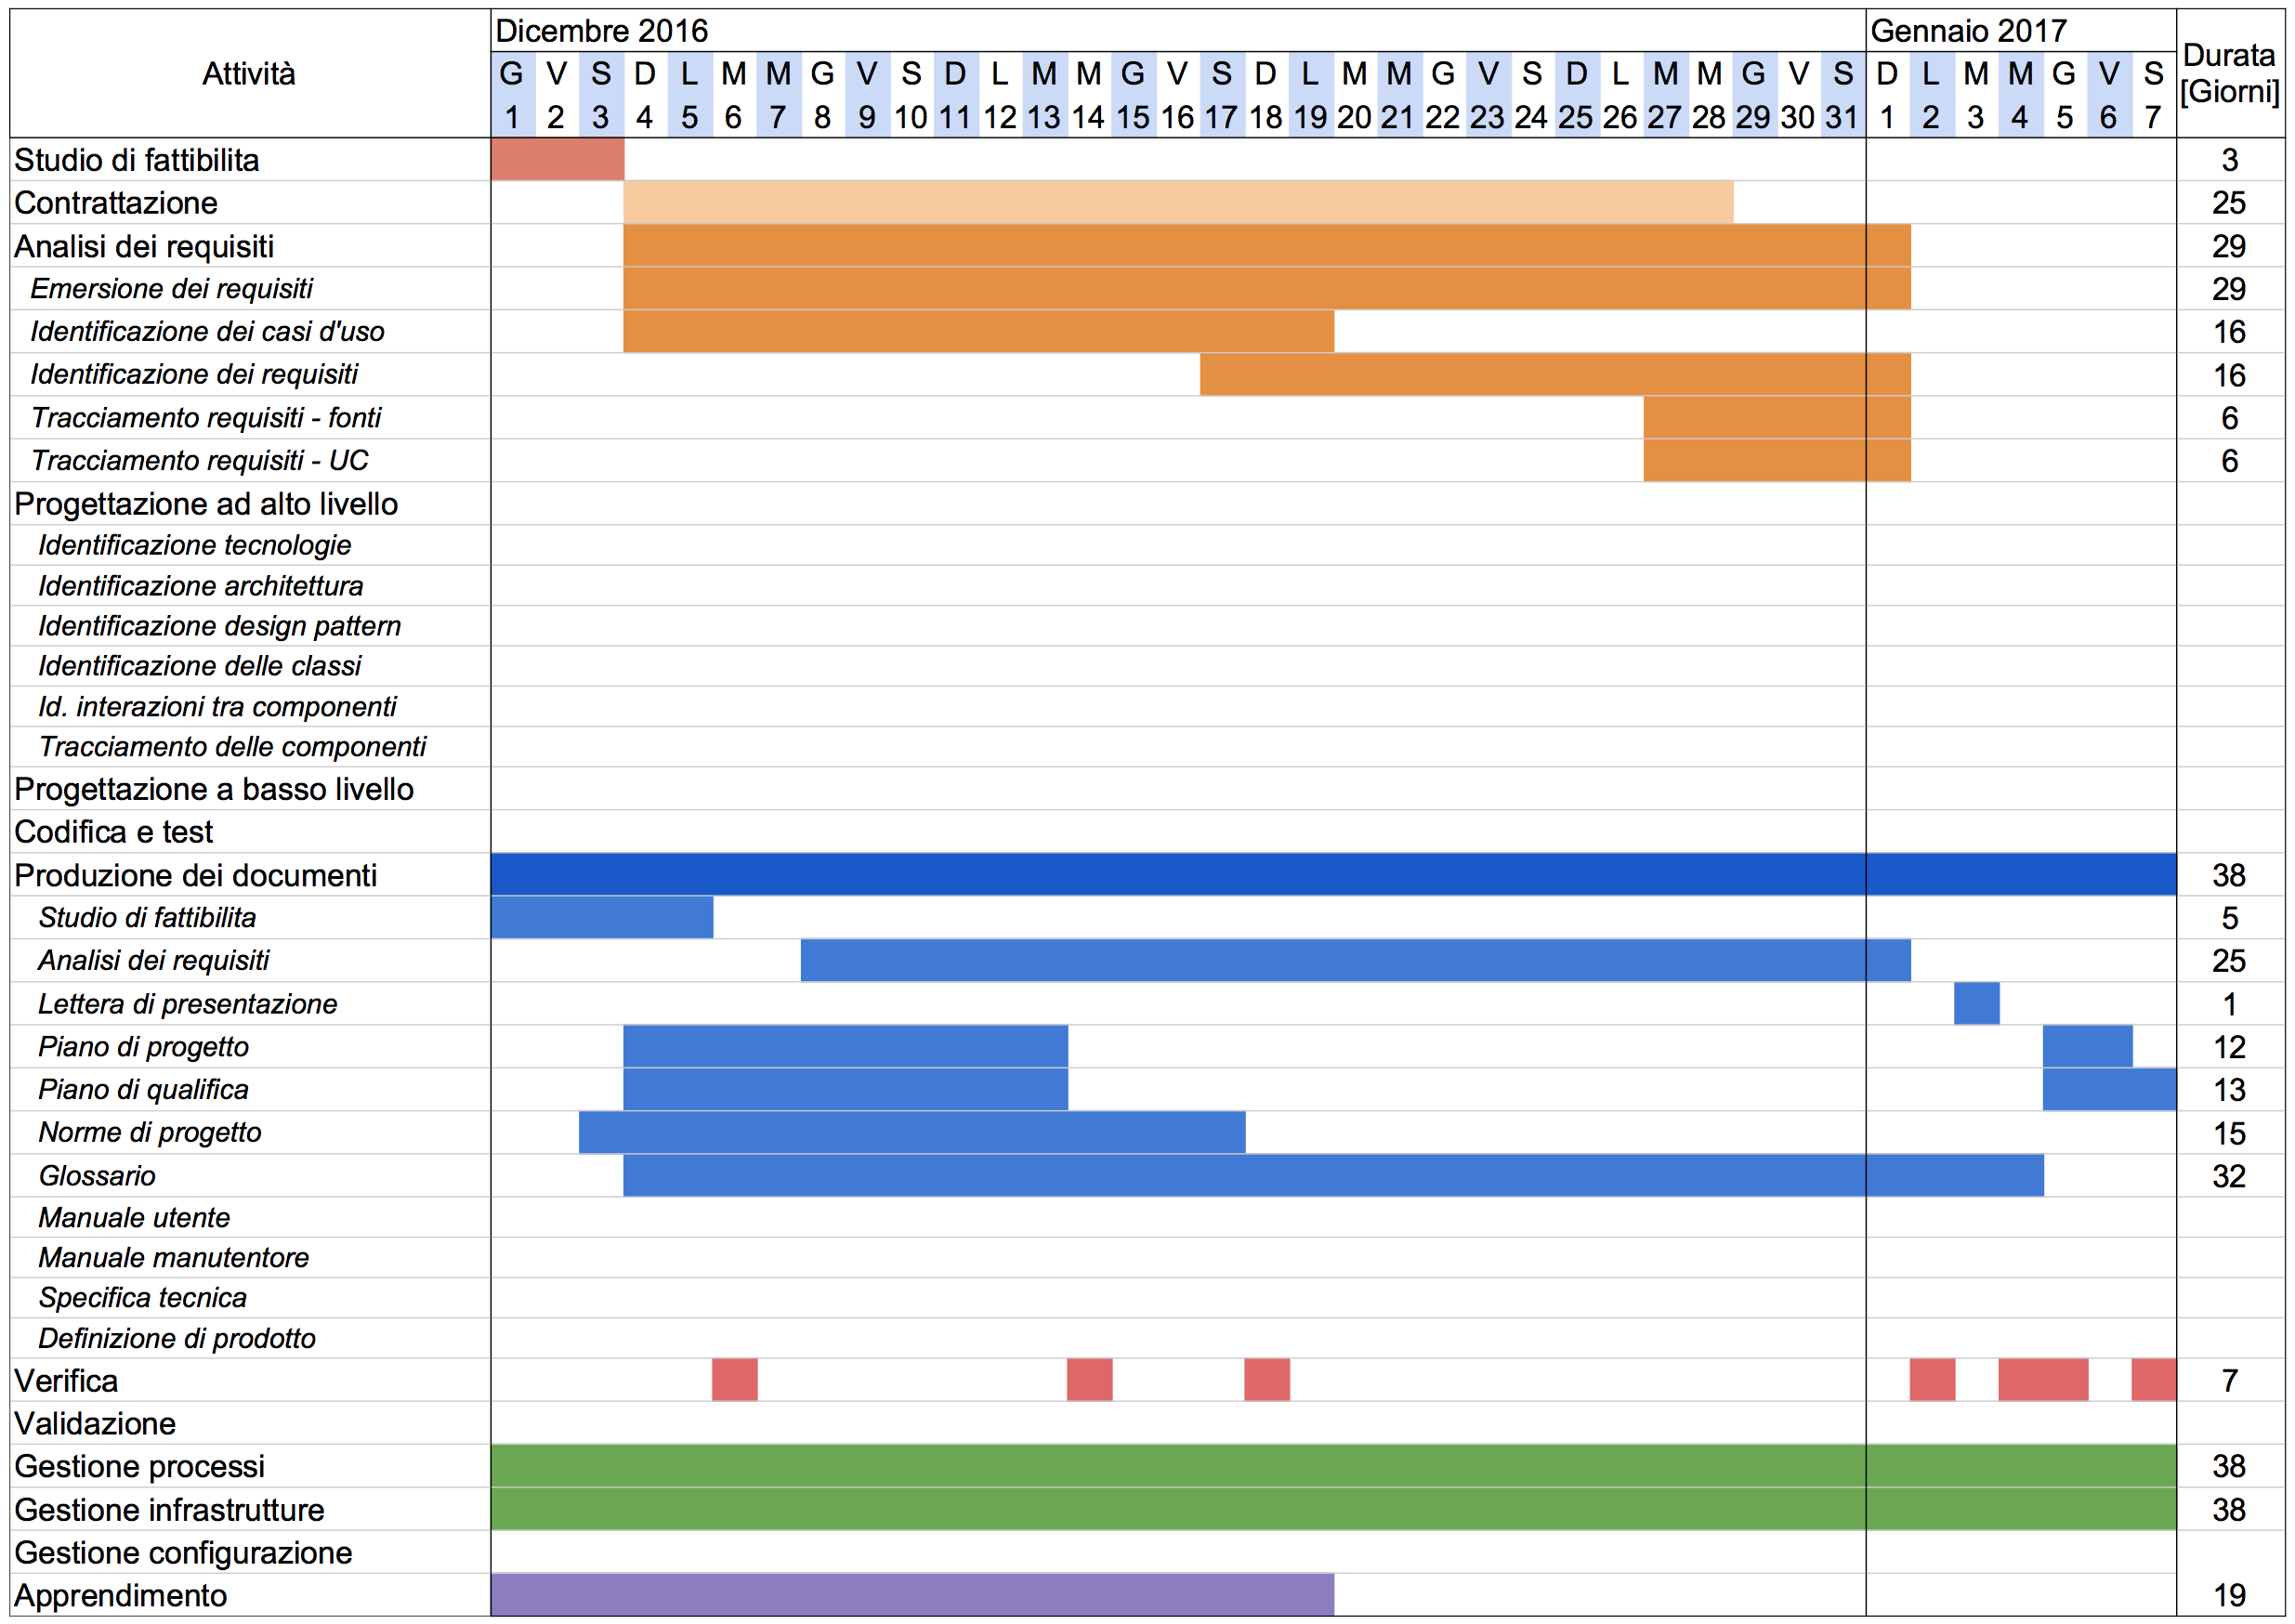
\includegraphics[width=\textwidth]{img/Gantt/g1c.png}
			\caption{Diagramma di Gantt - \glo{Periodo}{Periodo} di analisi}
		\end{figure}
		
	\newpage
	\subsubsection {Progettazione logica}
		\textbf{Periodo}: da \frmdata{12}{01}{2017} a \frmdata{02}{03}{2017} (50 giorni) \\
		Durante questo periodo:
		\begin{itemize}
			\item viene ultimata la raccolta di requisiti;
			\item vengono definiti gli incrementi;
			\item vengono assegnati i requisiti agli incrementi;
			\item viene stabilita l'architettura di massima del sistema.
		\end{itemize}
		Nel corso della progettazione logica verranno quindi individuati gli incrementi, che saranno riportati nel diagramma di Gantt del terzo periodo a partire dalla versione 2.0.0 del \pdp.
		\paragraph{Incrementi individuati}
		Durante il secondo periodo sono stati individuati i seguenti incrementi:
		\begin{itemize}
			\item incremento 1 - mappa;
			\item incremento 2 - \glo{Asset}{asset};
			\item incremento 3 - \glo{Nodo}{nodi};
			\item incremento 4 - \glo{Arco}{archi};
			\item incremento 5 - scenari;
			\item incremento 6 - analisi;
			\item incremento 7 - tutorial;
			\item incremento 8 - assistente vocale.
		\end{itemize}
		\paragraph{Assegnazione dei requisiti agli incrementi}
		Durante il secondo periodo i requisiti presenti nel documento di \adr sono stati assegnati agli incrementi elencati nel paragrafo precedente.
			\begin{table}[H]
				\centering
				\begin{tabular}{ll}
					\toprule
					\textbf{Requisiti}                           & \textbf{Incrementi}              \\
					\midrule
					ROF1 & 2 - asset \\
					ROF2 & 2 - asset \\
					ROF3 & 2 - asset \\
					ROF4 & 2 - asset \\
					ROF5 & 2 - asset \\
					\midrule
					ROF6 & 3 - nodi \\
					ROF7 & 3 - nodi \\
					ROF8 & 3 - nodi \\
					ROF9 & 3 - nodi \\
					ROF10 & 3 - nodi \\
					\midrule
					ROF11 & 4 - archi \\
					ROF12 & 4 - archi \\
					ROF13 & 4 - archi \\
					ROF14 & 4 - archi \\
					ROF15 & 4 - archi \\
					\midrule
					RFF16 & 5 - scenari \\
					RFF17 & 5 - scenari \\
					RFF18 & 5 - scenari \\
					RFF19 & 5 - scenari \\
					RFF20 & 5 - scenari \\
					\midrule
					RFF21 & 6 - analisi \\
					RFF22 & 6 - analisi \\
					RFF23 & 6 - analisi \\
					\midrule
					ROF24 & 1 - mappa \\
					\midrule
					RFF25 & 7 - tutorial \\
					\midrule
					RFF6  & 8 - assistente vocale \\
					\bottomrule
				\end{tabular}
				\caption{Assegnazione dei requisiti agli incrementi}
			\end{table}
		I requisiti non presenti in questa tabella sono da considerarsi implicitamente assegnati ad ogni incremento.
		\paragraph{Processi e attività coinvolte}
			\begin{table}[H]
				\centering
				\begin{tabular}{ll}
					\toprule
					\textbf{Processo}                           & \textbf{Attività}              \\
					\midrule
					\multirow{2}{*}{\textbf{Sviluppo}}          & Analisi dei requisiti          \\
					& Progettazione ad alto livello  \\
					\midrule
					\textbf{Documentazione}            & Produzione dei documenti       \\
					\midrule
					\textbf{Verifica}                  & Verifica                       \\
					\midrule
					\textbf{Gestione processi} 					& Gestione processi              \\
					\midrule
					\textbf{Gestione infrastrutture}				& Gestione infrastrutture        \\
					\midrule
					\textbf{Gestione della configurazione}				& Gestione della configurazione        \\
					\midrule
					\textbf{Apprendimento} 						& Apprendimento                 \\
					\bottomrule
				\end{tabular}
				\caption{Processi e relative attività}
				\label{Pl-ProcessiAttività}
			\end{table}
		\paragraph{Diagramma di Gantt}
		\begin{figure}[H]
			\centering
			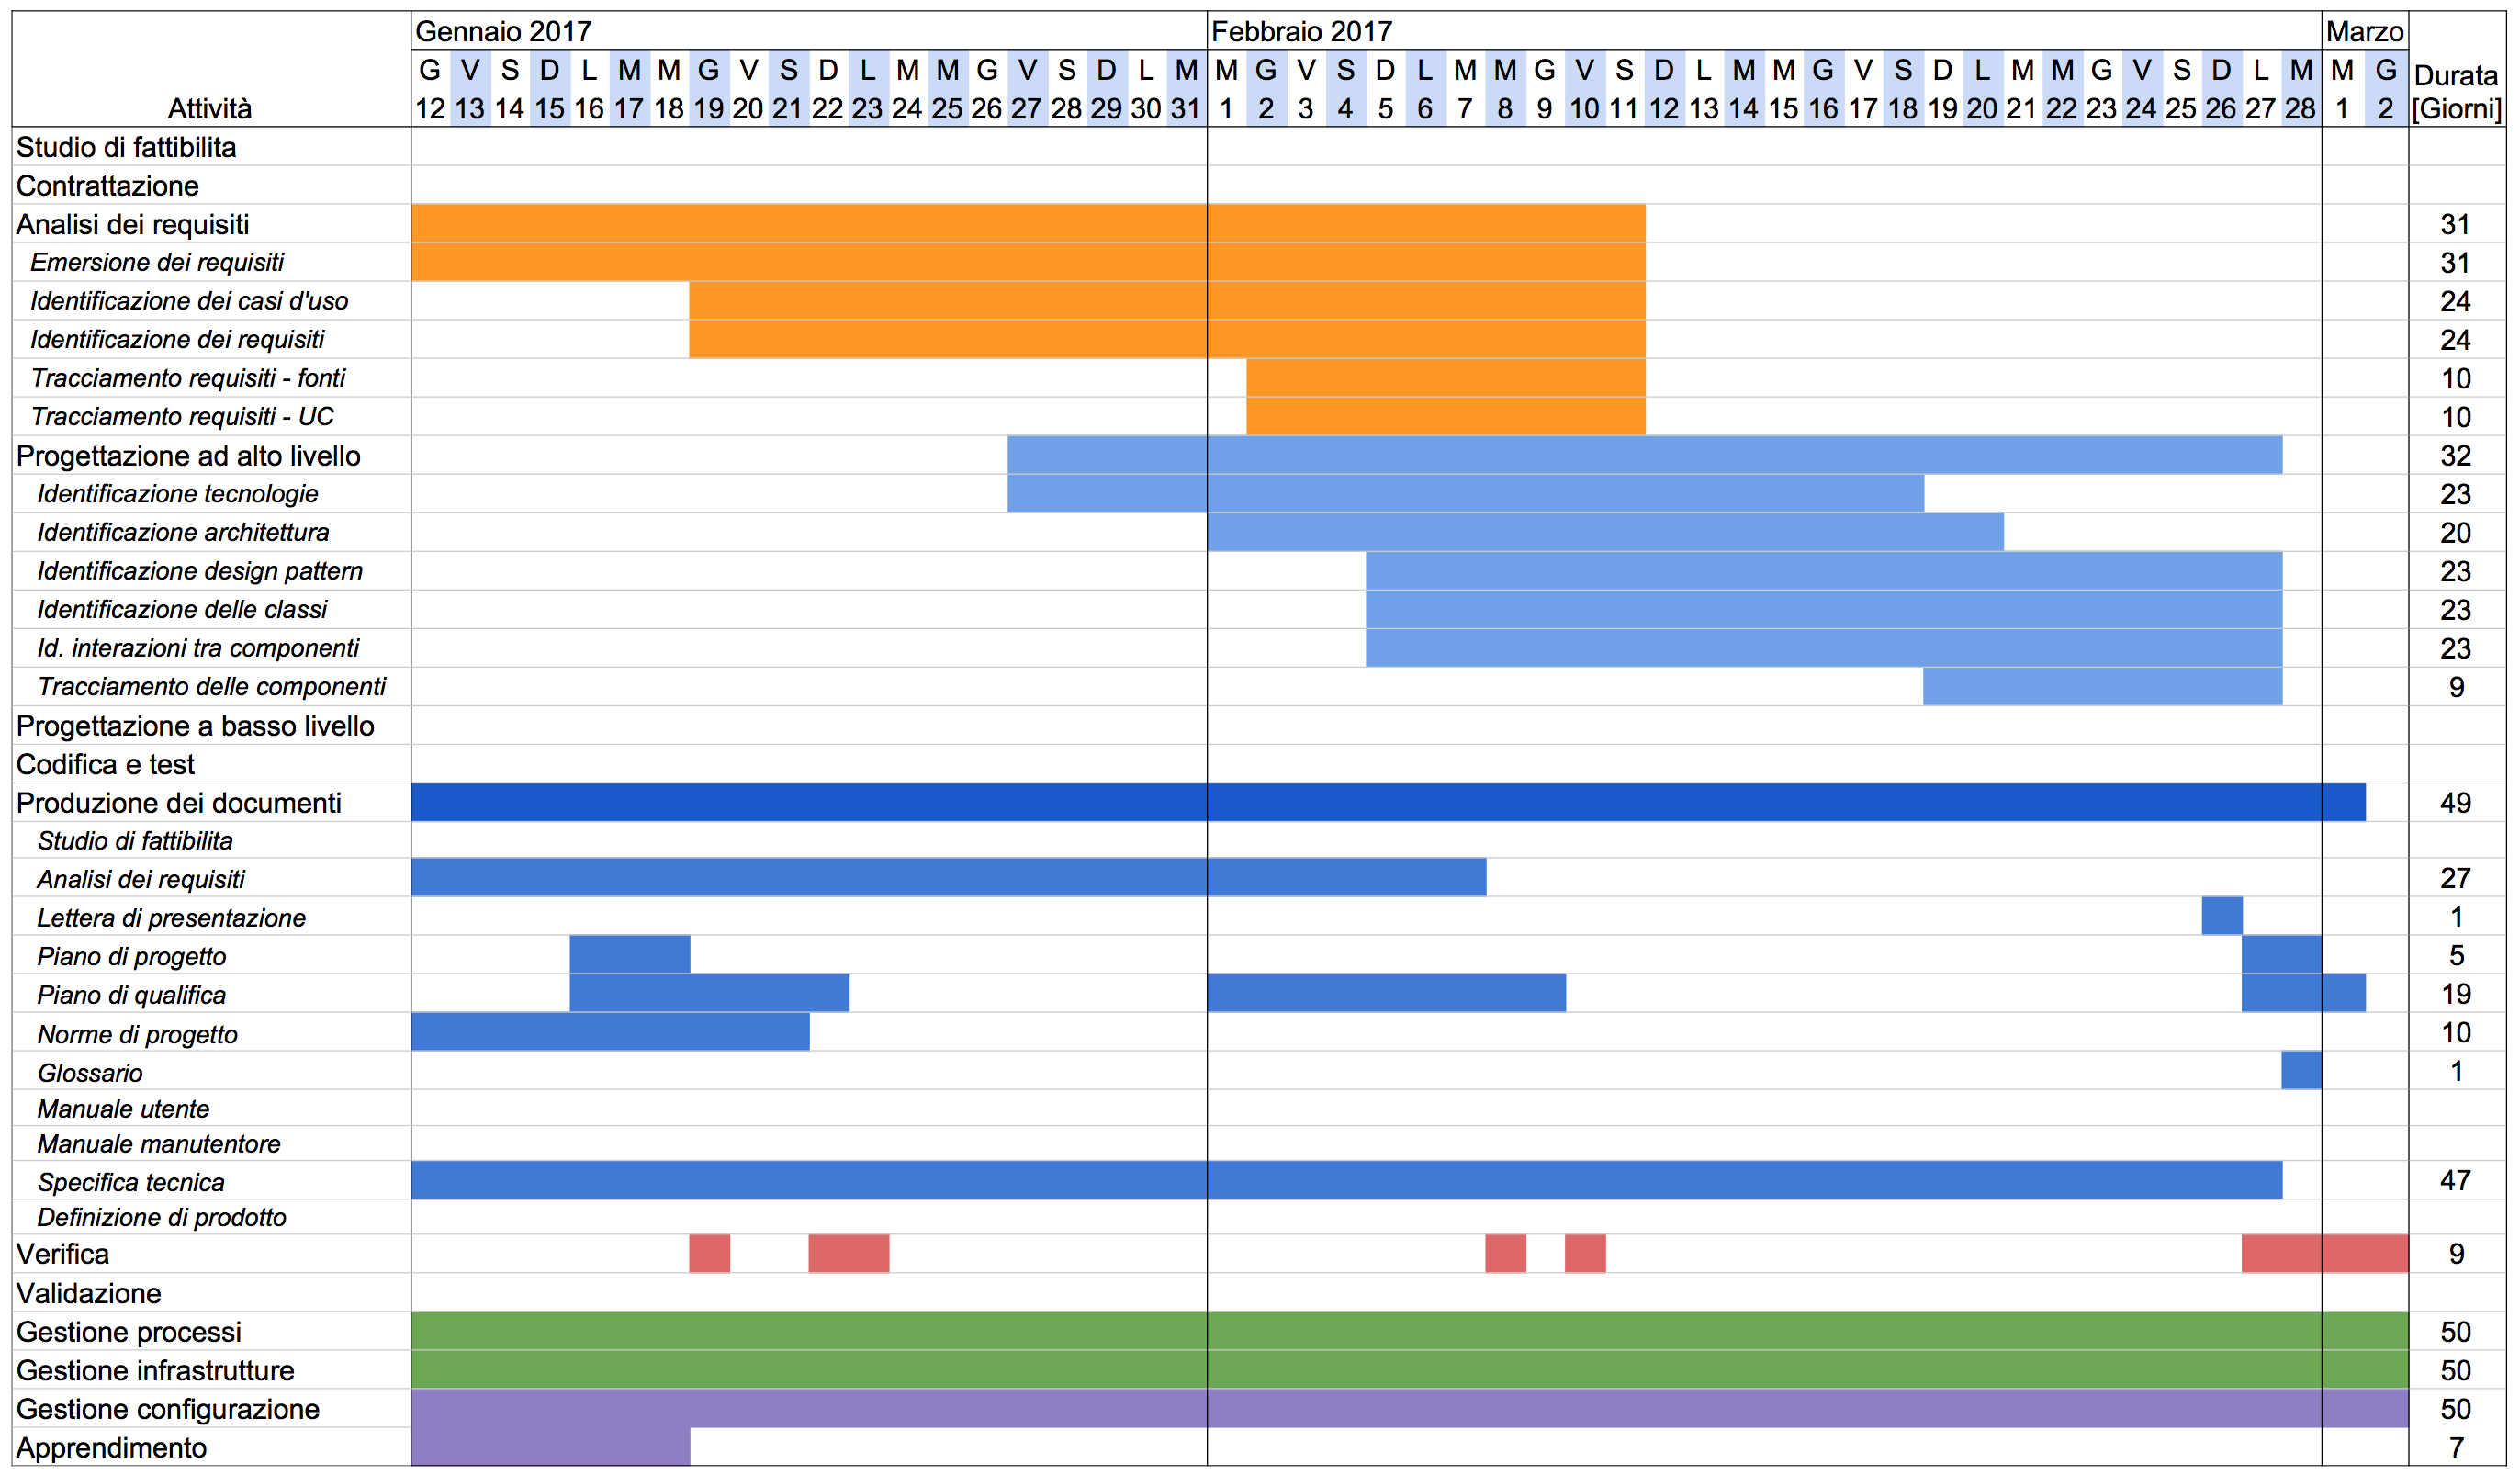
\includegraphics[width=\textwidth]{img/Gantt/g2c.png}
			\caption{Diagramma di Gantt - Periodo di progettazione logica}
		\end{figure}
	
	\newpage
	\subsubsection {Progettazione di dettaglio, codifica e validazione}
		\textbf{Periodo}: da \frmdata{07}{03}{2017} a \frmdata{07}{04}{2017} (31 giorni)\\
		Questo periodo consiste in un ciclo in cui ogni iterazione è data da progettazione, codifica, testing, integrazione del singolo incremento e dalla validazione dell'intero prodotto creato fino a quel momento.
		\\Una volta terminati tutti gli incrementi, il ciclo terminerà.
		\\Le linee verticali presenti nel diagramma indicano i rilasci del sistema validato alla fine dei vari incrementi.
		\paragraph{Processi e attività coinvolte}
			\begin{table}[H]
				\centering
				\begin{tabular}{ll}
					\toprule
					\textbf{Processo}                           & \textbf{Attività}              \\
					\midrule
					\multirow{2}{*}{\textbf{Sviluppo}}          & Progettazione ad basso livello \\
					& Codifica e test \\
					\midrule
					\textbf{Documentazione}            & Produzione dei documenti       \\
					\midrule
					\textbf{Verifica}                  & Verifica                       \\
					\midrule
					\textbf{Validazione}               & Validazione                    \\
					\midrule
					\textbf{Gestione processi} 					& Gestione processi              \\
					\midrule
					\textbf{Gestione infrastrutture}				& Gestione infrastrutture        \\
					\midrule
					\textbf{Gestione della configurazione}				& Gestione della configurazione        \\
					\midrule
					\textbf{Apprendimento} 						& Apprendimento                 \\
					\bottomrule
				\end{tabular}
				\caption{Processi e relative attività}
				\label{Pdrob-ProcessiAttività}
			\end{table}
		\paragraph{Diagramma di Gantt}
		\begin{figure}[H]
			\centering
			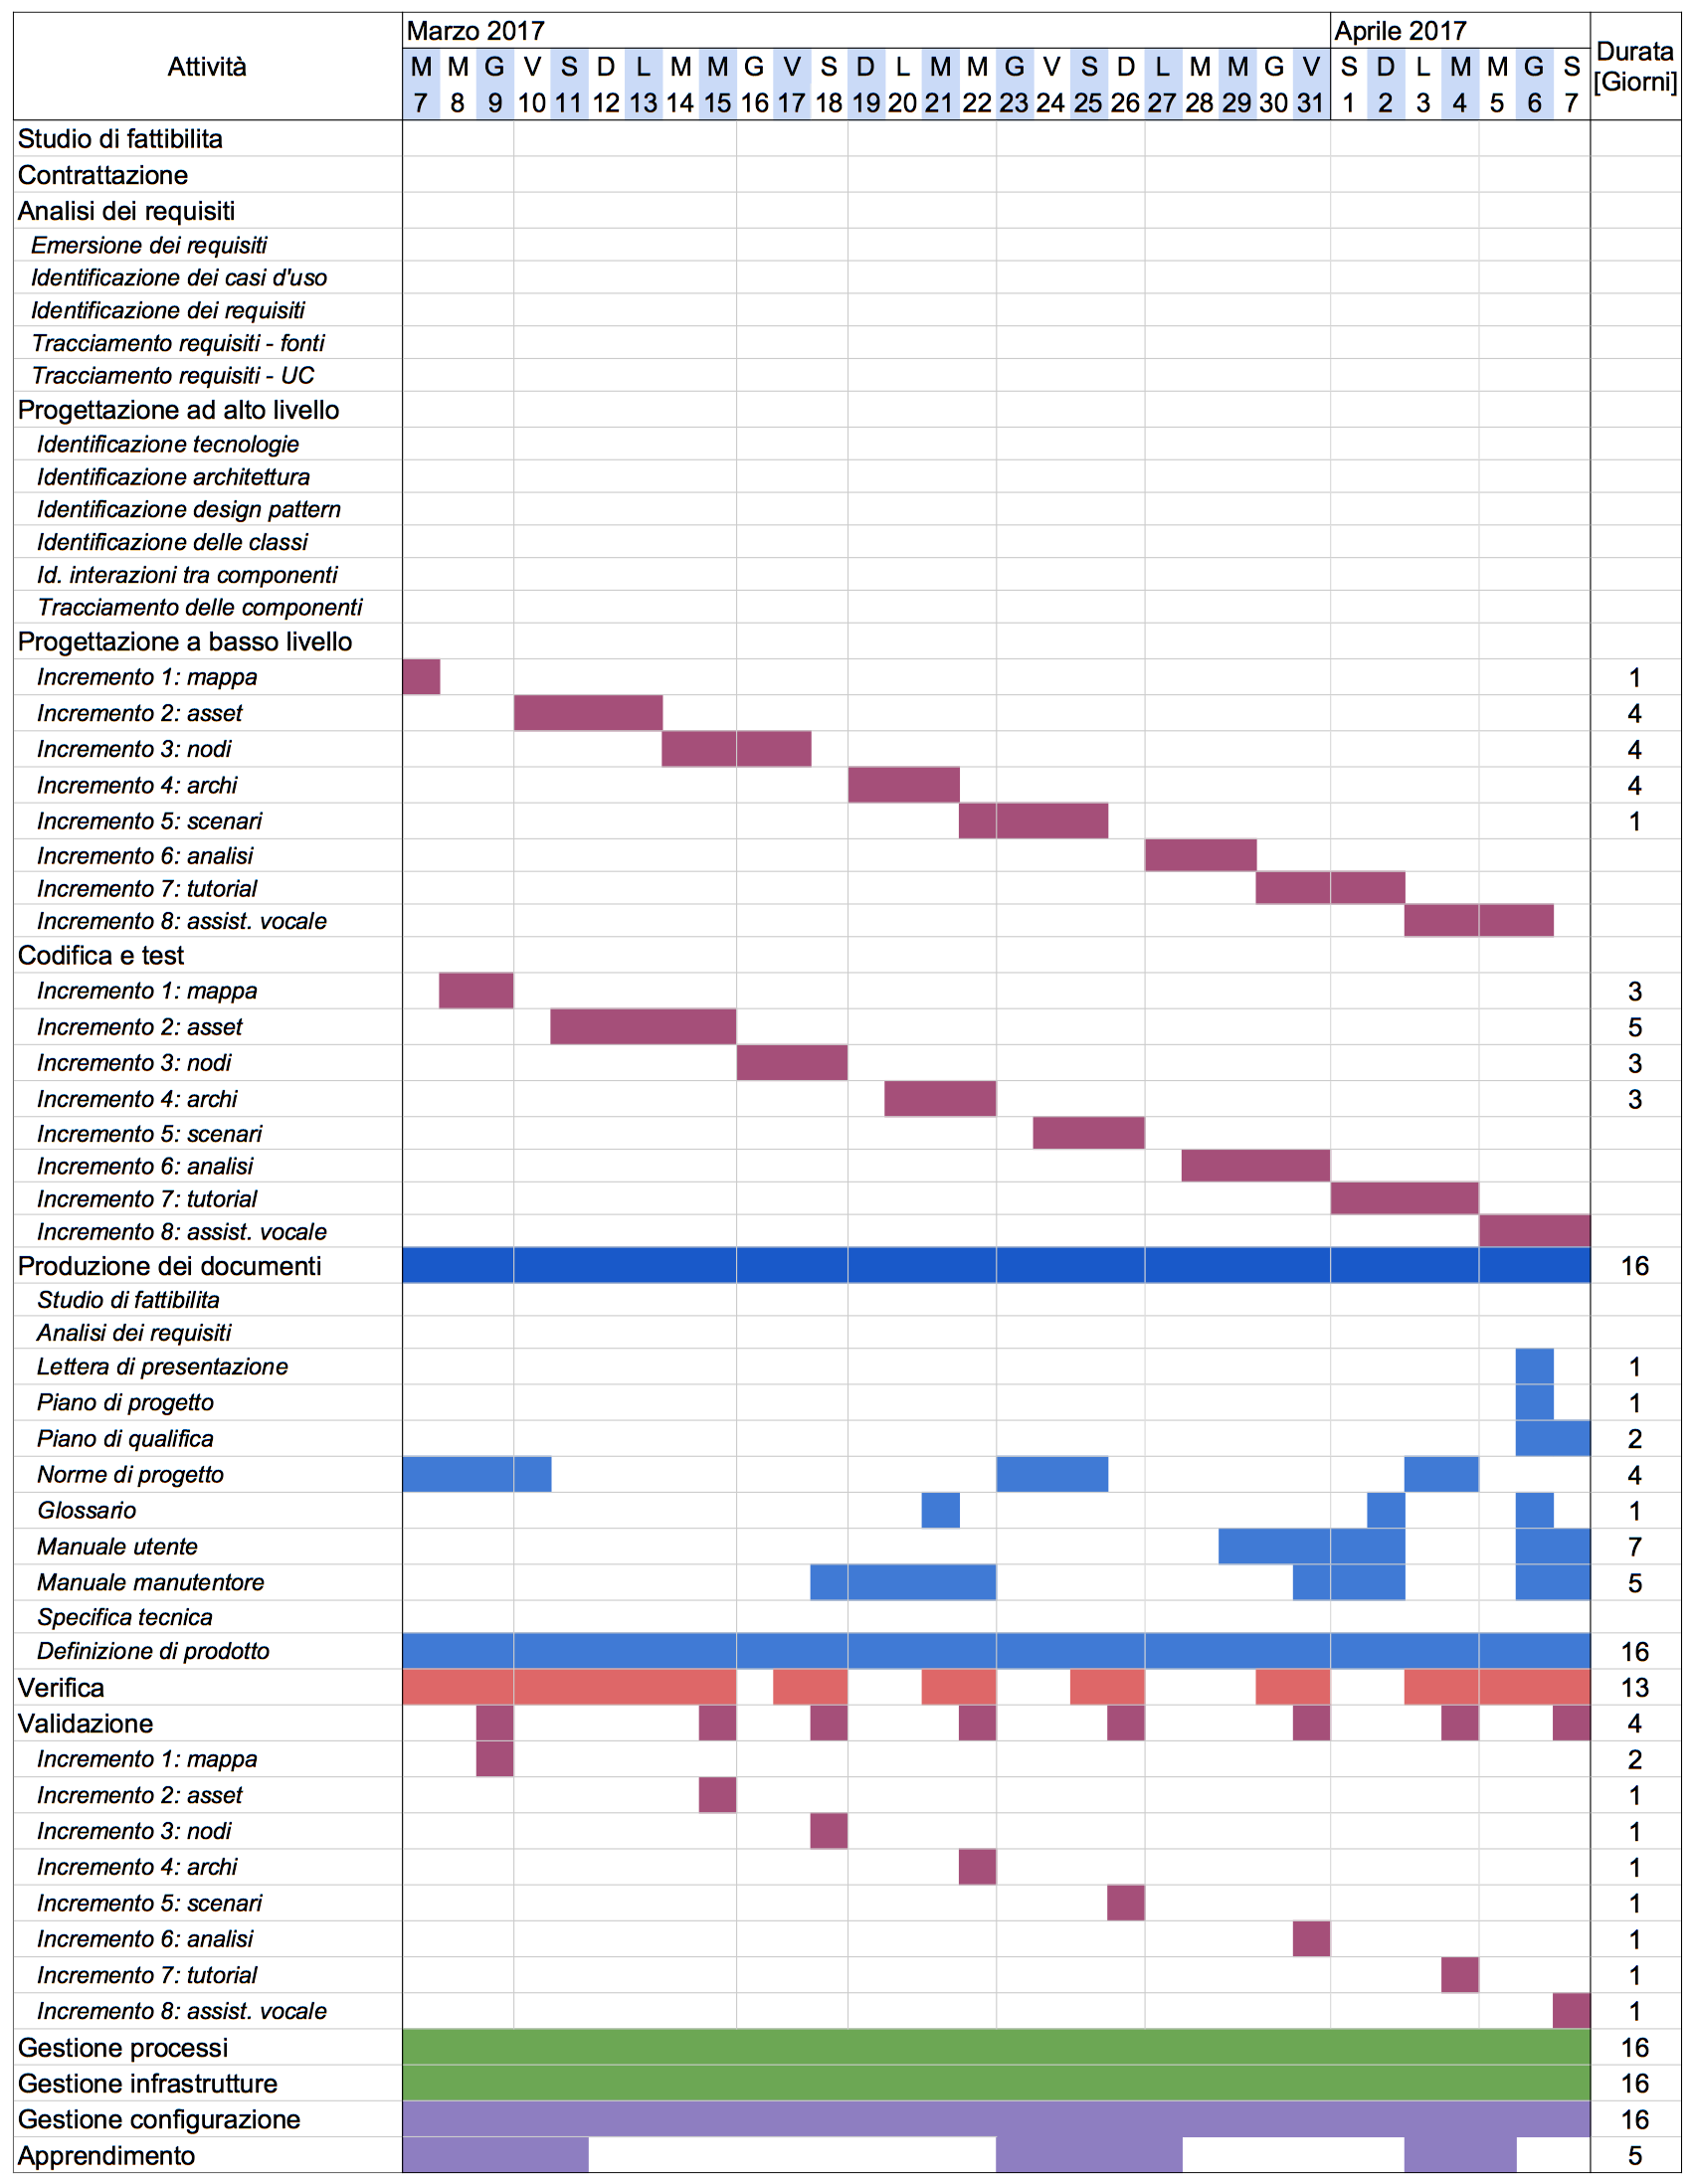
\includegraphics[width=\textwidth]{img/Gantt/g3c.png}
			\caption{Diagramma di Gantt - Periodo di Progettazione di dettaglio Codifica Validazione}
		\end{figure}
		
	\newpage
	\subsubsection {Validazione}
		\textbf{Periodo}: da \frmdata{12}{04}{2017} a \frmdata{04}{05}{2017} (23 giorni) \\
		Durante questo periodo si effettueranno i test di accettazione e il collaudo del sistema.
		\paragraph{Processi e attività coinvolte}
			\begin{table}[H]
				\centering
				\begin{tabular}{ll}
					\toprule
					\textbf{Processo}                           & \textbf{Attività}              \\
					\midrule
					\textbf{Documentazione}            & Produzione dei documenti       \\
					\midrule
					\textbf{Verifica}                  & Verifica                       \\
					\midrule
					\textbf{Validazione}               & Validazione                    \\
					\midrule
					\textbf{Gestione processi} 					& Gestione processi              \\
					\midrule
					\textbf{Gestione infrastrutture}				& Gestione infrastrutture        \\
					\midrule
					\textbf{Gestione della configurazione}				& Gestione della configurazione        \\
					\bottomrule
				\end{tabular}
				\caption{Processi e relative attività}
				\label{Va-ProcessiAttività}
			\end{table}
		\paragraph{Diagramma di Gantt}
		\begin{figure}[H]
			\centering
			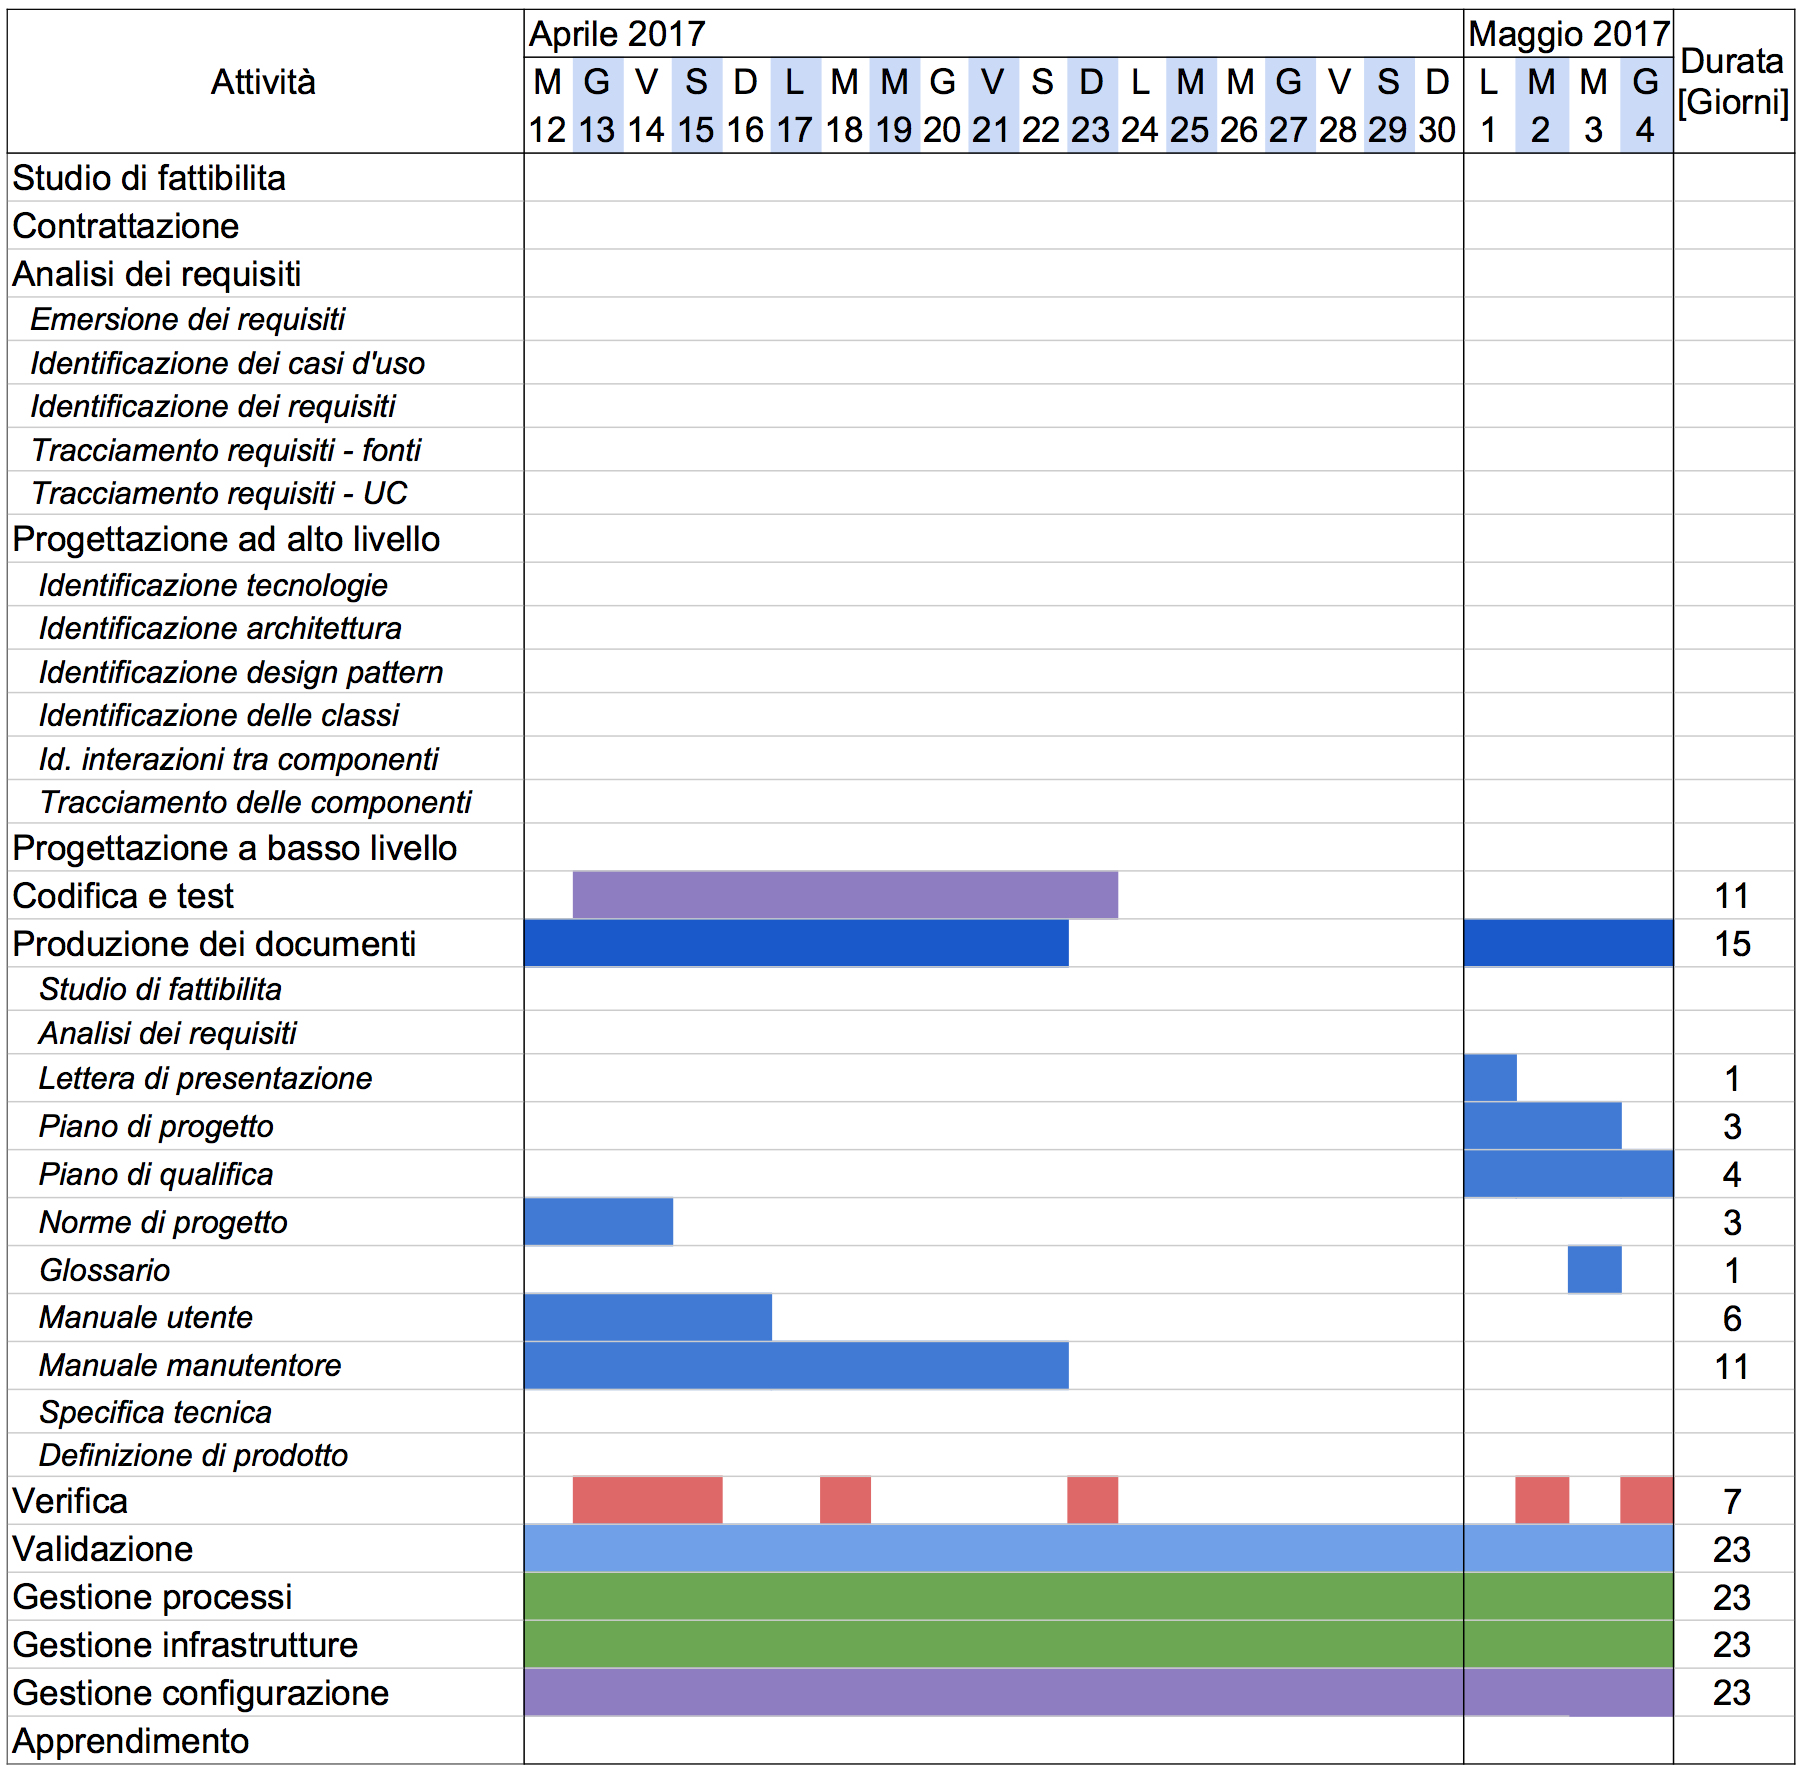
\includegraphics[width=\textwidth]{img/Gantt/g4c.png}
			\caption{Diagramma di Gantt - Periodo di validazione}
		\end{figure}
